\subsection{BMP085 Trykføler}

I forbindelse med læsning af sensordata fra den barometriske trykmåler BMP085, bruges I2C interfacet. Atmega32 understøtter I2C komunikatiuon og på figur~\ref{fig:voltagedivider} ses den hardwaremæssige opsætning. Atmega 32’s input spænding er 5V bruges en simpel spændingsdeler, så BMP085 ikke overbelastes.


\begin{figure}[h]
	\centering
	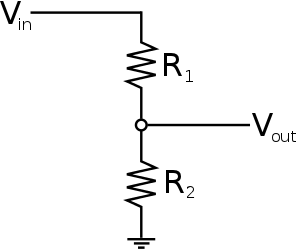
\includegraphics[width=0.3\linewidth]{figs/voltage_divider}
	\caption{Spændingsdeler.}
	\label{fig:voltagedivider}
\end{figure}

På figur~\ref{fig:voltagediv} vise modstandsberegningerne til spændingsdeleren.



\begin{figure}[h]
	\centering
	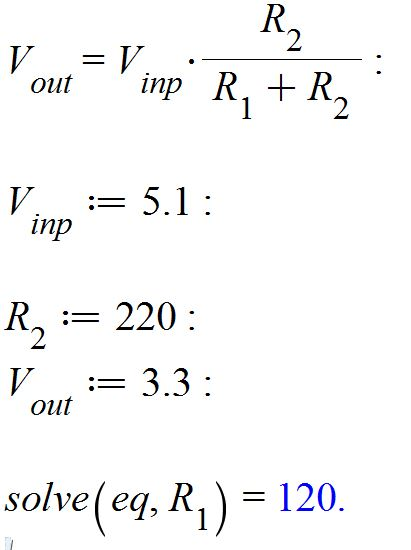
\includegraphics[width=0.3\linewidth]{figs/voltage_div}
	\caption{Spændingsdeler.}
	\label{fig:voltagediv}
\end{figure}

\subsection{Brug af I2C bussen med BMP085}

I2C protokollen implementerer master/slave teknikken, og er et TWI (two wire interface). 
Atmega32 agerer I2C master som sætter clock hastigheden ved at skrive til PIN (SCK). I2C masteren sender data bytes til I2C slaven på addressen 0x77.
Ifølge BMP085’s datablad er følgene kommandoer mulige:

\begin{figure}[h]
	\centering
	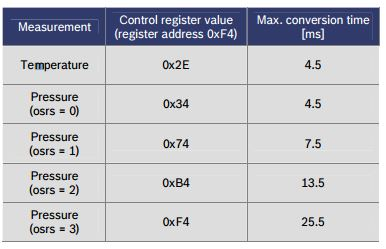
\includegraphics[width=0.6\linewidth]{figs/bmp085_commands}
	\caption{BMP085 kommandoer.}
	\label{fig:bmp085commands}
\end{figure}

Kommandoerne er definerede BMP085 driverens h-fil. Oversampling modes er defineret separat.

\begin{figure}[h]
	\centering
	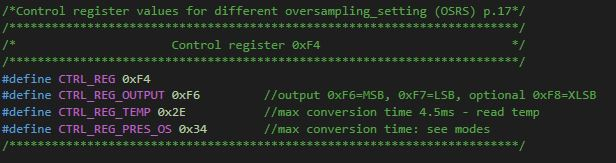
\includegraphics[width=0.7\linewidth]{figs/bmp085_command_defines}
	\caption{BMP kommandodefinitioer.}
	\label{fig:bmp085commanddefines}
\end{figure}

\begin{figure}[h]
	\centering
	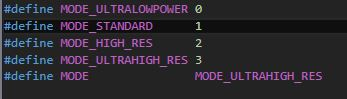
\includegraphics[width=0.7\linewidth]{figs/bmp085_command_modes}
	\caption{BMP085 kommendo tilstande.}
	\label{fig:bmp085commandmodes}
\end{figure}

Timing diagrammet for start af temperatur/tyk måling fremgår a BM085’s datablad, og kan ses på figur~\ref{fig:bmpi2ctiming}.

\begin{figure}[h]
	\centering
	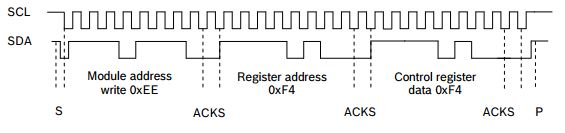
\includegraphics[width=0.9\linewidth]{figs/bmp_i2c_timing}
	\caption{BMM/I2C timingdiagram}
	\label{fig:bmpi2ctiming}
\end{figure}

Som det kan ses på figur~\ref{fig:bmpi2ctiming}, sender BMP085 en ACK for hver 8 bit der modtages. Atmega32 masteren sender en stop condition efter sidste ACK. S indikerer start conditionen.
Som angivet på figur~\ref{fig:bmp085commands} er der konverterings tider forbundet med målingerne. BMP085 giver muliged for at signalere et fuldendt måling ved at sætte BMP085’s EOC pin høj når en kovertering er slut. Dette bruges dog ikke i dette projekt da der ikke har været tid til at udvikle kredsløbet der hiver 3.3v logik op til 5v.

\subsection{Implementering af I2C driver}
Der er i dette projekt taget udgangspunkt i en I2C driver\footnote{Peter Fleury} til at initiere interfacet samt sende/modtage tage på I2C bussen.

Af hovedfunktionaliteter der benyttes kan der blandt andet nævnes:

\begin{itemize}
	\item Initiering af I2C bussen:
	\begin{itemize}
		\item Sætter clock hastigheden (uden prescaler).
	\end{itemize}
	
	\item Afsendelse af start condition:
	\begin{itemize}
		\item TWCR = (1<<TWINT) | (1<<TWSTA) | (1<<TWEN). TWI interrupt flagget cleares, start flagget sættes, TWI Enable sættes til 1.
	\end{itemize}
	
	\item Afsendelse af stop condition:
	\begin{itemize}
		\item TWCR = (1<<TWINT) | (1<<TWEN) | (1<<TWSTO);
		\item Herefter frigives I2C bussen.
	\end{itemize}
	
	\item Indlæsning af data
	\begin{itemize}
		\item Returnerer indholdet af TWDR. Hvis der ønskes yderligere data fra BMP085 sættes TWEA bitten (Acknowledge)
	\end{itemize}
	
\end{itemize}

\subsubsection{Fejlhåndtering i I2C driver}
Når en start condition sendes til BMP085 returneres 0 hvis den ikke er tilgængelig.

\subsection{Kalibrering af BMP085}
BMP085 har indkodet kalibrerings data i dens EEPROM, som bruges til at kompensere offsettet på udførte målinger. I alt indeholder EEPROM’en 176 bit kalibreringsdata der har til formål at tweake sensorens parametre og målinger\footnote{BMP085 Data Sheet rev. 1.2 side 8}. I I2C driveren findes en funktion til indlæsning af kalibreringsdata.
For at give en ide om kalibreringens virkemåde kan et pseudo kode eksempel ses nedenfor. 
Pseudokokde ekspempel på hvordan kalbreringsdata bruges til kompensering af temperatur-måledata i driveren.

\begin{lstlisting}
//Get calibration data
readMemory(CAL_REG_AC5, buffer, 2);
regAC5 = buffer[0] <<8 | buffer[1]));
readMemory(CAL_REG_AC6, buffer, 2);
regAC6 = buffer[0] <<8 | buffer[1]));

//calculate raw temperature
Ut = uncompensatedValue;
x1 = ut - regAC6) * regAC5 >> 15;
x2 = regMC << 11) / (x1 + regMD);
rawTemperature = x1 + x2;
\end{lstlisting}

Beregningerne understøttes af BMP085’s datablad på side 13.
BMP085 har ikke mulighed for at måle altitude. Dog kan dette beregnes da det gennemsnitlige tryk ved havoverfladen er kendt da ligningen på figur \ref{fig:equation} er givet.

\begin{figure}[h]
	\centering
	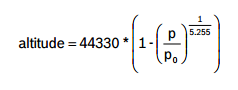
\includegraphics[width=0.45\linewidth]{figs/equation}
	\caption{Ligning.}
	\label{fig:equation}
\end{figure}

I driveren sættes $P_0$ til 101325 Pa, trykket aflæses fra måleren hvorefter altitude beregnes og returneres. 

\begin{figure}[h]
	\centering
	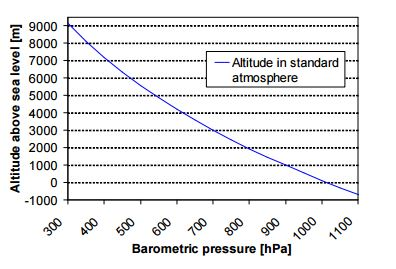
\includegraphics[width=0.7\linewidth]{figs/altitude_graph}
	\caption{Altitude graf.}
	\label{fig:altitude_graph}
\end{figure}

% The technical considerations and choices made during the project work.

% Advantages and disadvantages for the possible alternative solutions.

% How the group has acquired the knowledge necessary to do the project work.
